\documentclass[../main.tex]{subfiles}



\begin{document}

\section{Lecture 21}

\subsection{Quiz}

\pp{1}
Constrained Optimization
In a constrained optimization problem, when is the Hessian matrix of the Lagrangian function positive definite?

Hint: All diagonal entries of a SPD matrix must be positive.

\begin{solution}
    Recall that the hessian contains a zero on a diagonal (in fact a block of zeros), so that it cannot be positive definite.
\end{solution}

\pp{2}

\begin{center}
    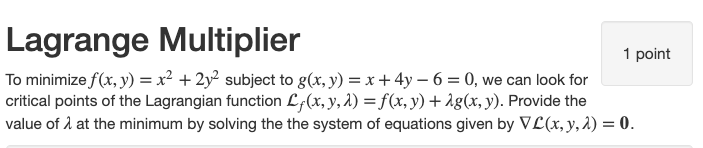
\includegraphics[width=\textwidth,height=\textheight,keepaspectratio]{lecture21_quiz_2}
\end{center}

\begin{solution}
    
    Recall what the lagrangian looks like rather than combine the terms and then differentiate.
\begin{center}
    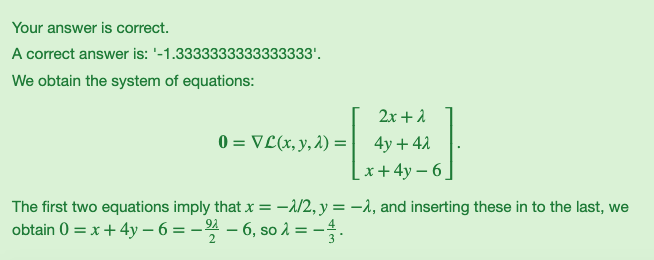
\includegraphics[width=\textwidth,height=\textheight,keepaspectratio]{lecture21_quiz_2_sol}
\end{center}
\end{solution}

\pp{3}

\begin{center}
    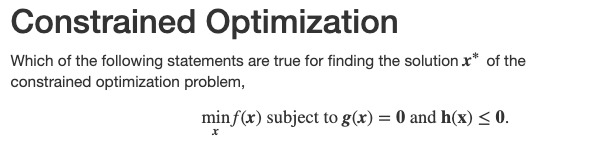
\includegraphics[width=\textwidth,height=\textheight,keepaspectratio]{lecture21_quiz_3}
\end{center}

$\nabla f(\xa) = 0$ \\

$\xa$ is a critical point of the Lagrangian function. \\

Sequential Quadratic Programming may be unreliable unless it starts close to the solution. \\

The inequality constraint $h(x)$ is only active on the interior of the feasible set.

\begin{solution}

    We know that a first order optimality condition is simply that $\nabla f(\xa)^T s \geq 0$, so the first answer cannot be correct(actually, the fist answer cannot be correct because KKT tells us that $\nabla_x(L, \lambda_1, \lambda_2) =  0$ and not $\nabla f(\xa) = 0$; we know that $\xa$ is a critical point of the Lagrangian by definition; SQP may be unreliable unless it starts close to the solution, precisely because SQP is Newton, which may fail if we don't apply it close to the solution.

    The last choice needs to be examined more closely.

    In general, for $h$ to be a non trivial constraint there has to be a point (and hence a neighborhood) where $h(x) > 0$ (this means that some $h_i$ gives $h_i(x) > 0$). It follows that by continuity there is a sequence of points $\{x_n\}$ such that $h(x_n) \to 0$, meaning that $x_n \to $ some point $z \in \inv{h}(0)$. It follows that $z$ must be some point on the boundary. UNRESOLVED

    We can design a function $h$ so taht $h(x) = 0$ and there exists a neighborhood at $x$ called $C$ such that there exist $c_1$ and $c_2$ such that $h(c_1) > 0$ and $h(c_2) < 0$.
    
    Just take $h: \R \to \R$ where $h(x) = x$ and consider $x = 0$.
\end{solution}

\pp{4}

Inequality Constrained Minimum \\
Find the optimal parameters and $\lambda$ inside the feasible set for the minimization function $f(x,y) = 5x^2 + 3y$ and $x+y \geq 5$.
\begin{solution}
    Form the lagrange function, which is

    \[
        5x^2 + 3y + \lambda(-x  -y +5)
    \]

    Then solve for $x,y, \lambda$ such that $\nabla_{L} = \mathbf{0}$.

    After you solve for the parameters, tweak them so that $x + y \geq 5$.

    Note that, in general, one would apply Newton's method (or a similar
    optimization scheme) to try and determine the minimum of $\nabla_{L}$.
\end{solution}

\pp{5}
Sequential Quadratic Programming
Which of the following are true about sequential quadratic programming (SQP)?

Select all that apply:
A single iteration of conjugate gradient suffices for each step of SQP
Each iteration of SQP requires a single iteration of Newton's method
SQP is more effective at handling inequality constraints than equality constraints
When dealing only with equality constraints, SQP is Newton's method for optimization

\begin{solution}
    \begin{outline}
        \1 Conjugate gradient is not used in SQP -- Newton's method is.
        \1 Yes, this is true -- by definition.
        \1 yes, for Heath explains that when we use inequality constraints, at a given iteration, we consider those constraints that are active and include
        them in the Lagrangian to which we then apply Newton's method.
        \2 For reasons that are not explained, this complication of having varying lagrangians that we minimize is less effective than simply using one, non-varying
        Lagrangian throughout the course of the problem.
        \1 Yes, indeed -- when we don't have inequality constraints, we are simply evertime computing $H_{L}(x) s = - \nabla_{L}(x)$ for $s$
    \end{outline}
\end{solution}






\begin{definition}
    An interpolatio problem asks us to find a function $f$ such that given a set of points $\{ (x_i, y_i) \}$ it holds that $f(x_i) = y_i$ for all $i$.
\end{definition}

\begin{definition}
    Suppose that we define $f = \sum_{i=1}^{n} \phi_{j}(x) \alpha_j$. Then$f(x_i) = y_i = \sum_{k=1}^{n}\phi_{k}(x_i) \alpha_k$.

    This can be framed as solve for $\alpha$ in 

    \[
        Y = V \alpha
    \]

    where $V_{i,k} = \phi_{k}(x_i)$ and $Y$ has all the solutions.
    
    If we require $V$ to be square, and hence there to be precisely
    as many basis functions as there are points $n$ -- then the 
    system above admits a unique solution in the event that $V$ is full rank.
\end{definition}

\begin{definition}
    When we use a monomial basis we ask to solve for $(x_1 \dots x_n)$ such that


    \[
        p(t) = \sum_{j=0}^{n-1}x_{j+1}t^{j} = y_{j+1}
    \]

    where $\left( (t_1, y_1) \dots (t_n,y_n) \right)$ are the function points.

    To solve for the $x$, we can solve the following system


    \[
        \begin{bmatrix}
            1 & t_1 & t_1^2 \dots (t_1)^{n-1} \\
            1 & t_2 & t_2^2 \dots (t_2)^{n-1} \\
            \vdots \\
            1 & t_n & t_n^2 \dots (t_n)^{n-1} \\
        \end{bmatrix} t = y
    \]

    Suppose that $Vz = 0$ where $z$ is some vector. This implies that a polynomial of degree $n-1$ has $n$ roots (ie $t_1 \dots t_n$), which can only take place if the resulting polynomial is the zero polynomial, which implies that $z = 0$. This tells us that under this basis, there necessarily exists an interpolant.
\end{definition}
\begin{definition}
    Lagrange interpolation seeks to make a basis $V$ that is the identity matrix. To that end we define

    \[
        \phi_j = \frac{\prod_{i \not = j}(x - x_i}{\prod_{i \not = j}(x_i - x_j)}
    \]

    Then observe that $\phi_j(x_j) = 1$ and that $\phi_j(x_i) = 0$ for any $i \not= j$.
\end{definition}

\begin{definition}
    Newton polynomials are obtained by using the basis function

    \[
        \phi_{j}(x) = \prod_{k=1}^{j-1}(x - x_k)
    \]

    where $\phi_1  = 1$. As a consequence, this gives us a matrix
    that is lower triangular.

    Finding the $\alpha$ vector then is an $O(n^2)$ process.

\end{definition}

\begin{remark}
    The conditioning of determining an interpolant via a basis matrix is approximately the conditioning of the underlying linear system. We need to also pay attention, however, to the behavior of the interpolant at points other than the nodes, for it should not be the case that an interpolant swings wildly at other points. This is foramlzied by saying that:

    \[
        \max_{x \in [a,b]} \abs{f(x)} \leq \Lambda_i \norm{y}_{\infty}
    \]

    where $\Lambda$ is a constant that depends on the points chosen for the interpolant, the basis of functions, and (we're working with polynomials of degree at most $i$), then the degree $i$.

    In general, for polynomials, since all bases give all possible polynomials, the constant solely depends on the points and the maximal degree $i$.
\end{remark}


\begin{definition}
    Polynomials are orthogona iff over an interval (for example $[-1,1]$), given some
    weight function $w(x)$, we have

    \[
        \int_{-1}^{1} f(x) g(x) w(x) = 0
    \]

    This can be shown to induce an inner product and, hence, we can invoke Gram Schmidt
    on a collection of $n$ polynomials to obtain a basis for $\mathbb{P}_{n-1}$, the 
    vector space of all polynomials of degree $n-1$.
\end{definition}

\begin{remark}
    This is useful, because if our interpolants constitute a basis, then we can be assured that we are representing as many functions as possible; it also turns out to be true that
    when we solve the normal equations $V a = y$ where $V$ is the vandermonde matrix, the matrix $V^TV$ is diagonal (UNRESOLVED: there is some matrix that -- according to Heath -- ends up being diagonal, but it is not known whether this is $V^TV$). Orthogonal polynomials also satisfy a three term recurrence, making computation of successive polynomials tractable.
\end{remark}

\begin{definition}
    In one special case, if we let the basis functions be

    \[
        \phi_j(x) = \cos(j \inv{\cos}(x))
    \]

    and we use equispaced points as our nodes, ie we use

    \[
        x_i = \cos\left( \frac{i}{k}\pi \right)
    \]

    then the entries of the vandermonde matrix, say $V_{i,j}$ end up being

    \[
        \cos\left( j(i/k)\pi \right)
    \]

    It can be shown that the mat-vec of the resultant matrix by any other vector is an $n \log n$ process. This is somehow related to the fourier transform. There are other useful properties of the chebyshev polynomials that Heath discusses.
\end{definition}

\section{Lecture 23}
\subsection{Quiz}

\pp{2}

see the code below that is commented and hence won't appear on th erendered page
%>>> def f(n):
%...  return np.pi**n/(2**(n+2) * (n-1)**n * n)
\pp{3}

Let hte interpolant be $a_0 + a_1 x$.
\[
    \implies a_0 + a_1(41.08) = 1.5945575554
\]

\[
    \implies a_0 + a_1(41.09) = 1.5944984844
\]

Solve for $a_0$ and $a_1$


%>>> A = np.asarray([[1, 41.08],[1, 41.09]])
%>>> b = np.asarray([1.5945575554, 1.5944984844])
%array([ 1.83722122, -0.0059071 ])

%Fuck it's just the average: Indeed , using the found coefficients above
will give us an ouput that is less than $f(41.08)$.
\[
    
\]

Suppose that we estimate a function using linear interpolation. The error is then bounded by:

\[
    \frac{f''(\zeta)}{2!}h^n
\]

Nah use the bound $h^n C M$ and take $C$ and $M$ to be $1$ and $h$ is by definition the distance between endpoints of the interval, which in this case is $0.04$.

\pp{5}
Assume that the error bound is given by

\[
    h^n CM
\]



\begin{remark}
    We jsut learned that the error of any interpolant which is a polynomial to a function $f$ where $p$ is at most of degree $n-1$ satisfies the result that the error $p_{n-1}(x) - f(x)$

    \[
        = \frac{f^{n}(\zeta)}{n!}\prod_{i=1}^{n}(x -x_i)
    \]

for some $\zeta  \in I$, which is a closed intervable on which $f$ is $n$ times continuously differentiable.
\end{remark} 
We can use this to obtain a generic error bound on our interpolant:

Assume that $x_i \in [x_1, x_n] = h$. Then 

\[
    \max \abs{p_{n-1}(x) - f(x)} \leq h^n \frac{f^n(\zeta)}{n!} = h^n \frac{MC}{1}
\]

where we assume that $f^{n}(x) \leq M$ for all $x \in I$ and $C$ is some constant independent of $h$.


\begin{remark}
    How to perform piecewise polynomial interpolation of degree $n$.

    \begin{outline}
        \1 Assume that we're given two points $(x_1, y_1)$ and $(x_2, y_2)$ for one interval and that there are $N$ intervals. Then form the interpolant:

        \[
            a_0 + a_1x + a_2x^2 + \dots a_{n}x^{n} = f(x)
        \]

        and solve for $a_i$ using $f(x_1) = y_1$ and $f(x_2) = y_2$.
        \2 In general, observe that there will be $(n+1)(N)$ unknowns.
        \3 For cubic splines, there are $4N$ unknowns
        \2 This gives us two equations for one interval.
        \3 In total, there fore we have $2N$ equations here.
        \1 Add some smoothness conditions -- ie the derivative of the polynomial in one interval must agree with the derivative in the next interval and we get more equations. Make this hold with respect to second derivatives as well.
        \2 This gives us $2(N-1)$ equations.
        \3 Finally require that the second derivatives be zero at each of the endpoints.
        \4 This gives us $2$ equations.
        \2 At this point, we have $4N$ equations. If we're working with cubic splines, then we have as many unknowns as equations and we can proceed to solve the system.
        \3 This construction above is called a cubic spline
    \end{outline}

\end{remark}

\section{Lecture 24}{Composite Quadrature and introduction to differentiation}


\begin{definition}
    In a composite quadrature rule, we take an interval with endpoints
    $a,b$ we subdivide it into $k$ intervals; then we interpolate
    over these $k$ intervals, each interval having its own interpolant.
    Using these interpolants, we then construct integrals.
\end{definition}

\begin{remark}
    Suppose that inside an interval, we use $n$ points and that
    the interval is open -- then we will need $kn$ interpolation points.
    On the other hand, if we interpolate over closed intervals,
    then we will need $(n-1)k + 1$ points. Why? For suppose that
    the closed interval is first really an open interval, meaning
    that it requires $kn$ points. Now correct our mistaken 
    assumption, by realizing that we have overcounted some
    points. In fact, we have over counted those points on the
    boundaries of intervals, each point exactly once -- there
    are $k-1$ such points so the total number of points needed
    is really $kn - (k-1) = (n-1)k + 1$.
\end{remark}

\begin{example}
    Suppose that we divide an interval into $k$ parts, each part
    solely containing two points and that
    the first point is $a$, the last point $b$, and points in
    between are given by $x_j = a + (b-a)/k j$ from $j = 0$ up
    to $j = k$. Then we apply the composite midpoint rule we find
    that the approximation is

    \[
        \sum_{j=0}^{k-1}f(\frac{x_{j} + x_{j+1}}{2})(x_{j+1} - x_{j})
    \]

    \[
        = h \sum_{j=0}^{k-1} f(\frac{x_{j} + x_{j+1}}{2})
    \]

    We can similarly derive the composite trapezoid rule.
\end{example}

The following is not proven (although shown in Heath 8.3.5):

\begin{proposition}
    In the limit -- as we use more and more subintervals of equal length -- provided
    that the underlying quadrature rule is stable, composite
    quadrature gives us an approximation to the integral.
\end{proposition}

\begin{unresolved}
    Do all interpolation formulas give the same interpolant?
\end{unresolved}<++>
\end{document}







